\documentclass{beamer}
\usepackage[spanish]{babel}
\usepackage[utf8]{inputenc}
\usepackage{multicol} % indice en 2 columnas
\usepackage{graphicx}
\usepackage{enumitem}
\usepackage{xcolor}
\usepackage{adjustbox}
%configura la figura de las listas itemize
\setlist[itemize]{label={\color{blue}$\bullet$}}
\usetheme{Warsaw}
\usecolortheme{dolphin}
\useoutertheme{shadow}
\useinnertheme{rectangles}

% 1º ppt
\title[IPv6]{Migrando aplicaciones a IPv6}
\subtitle{Fundamentos técnico: DualStack y Socket.h}
\author[Sandoval, Vargas]
{Alonso Sandoval A. \and Hernán Vargas L.}
\institute[UTFSM]
{
	Universidad Técnica Federico Santa María
	\and
	\texttt{asandova@alumnos.inf.utfsm.cl, hvargas@alumnos.inf.utfsm.cl}
}
\date{\today}

%2º ppt
\AtBeginSection{
	\begin{frame}
		\frametitle{Índice}
		\tableofcontents[currentsection]
	\end{frame}
}

\AtBeginSubsection{
	\begin{frame}
		\frametitle{Índice}
		\tableofcontents[currentsection,currentsubsection]
	\end{frame}
}

\begin{document}

\frame{\titlepage}

\begin{frame}
	\frametitle{Índice}
	\tableofcontents
\end{frame}

%tex_origin: ppt.tex
\section{Dual Stack Lite (DSL)}
\subsection{Métodos}

\begin{frame}
  \frametitle{Paquetes IPv4 bajo IPv6}
  \begin{columns}[t]
    \column{0.5\textwidth}
    	\begin{figure}
		\centering
		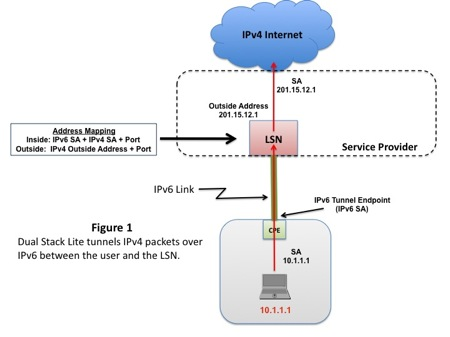
\includegraphics[width=150px]{img/img1.jpg}
	\end{figure}
    \column{0.5\textwidth}
    	\begin{itemize} %[itemsep=2em] 
		\footnotesize
		\item
			Cuando el cliente envía mensajes IPv4 se
			encapsulan en paquetes IPv6.
		\item
			En el LSN(Large Scale Nat) el paquete de 
			des-encapsula y NAT44 (Network address 
			translate for IPv4) actúa a continuación.
		\item
			La funcionalidad se implementa en el LSN.
		\item
			Para identificar cada equipo se realiza un mapeo
			que se guarda en una tabla con la siguiente 
			combinación: IPv6 address + IPv4 address + Port
	\end{itemize}
  \end{columns}
\end{frame}

\begin{frame}
  \frametitle{Paquetes IPv4 bajo IPv6 - Generalización}
  \begin{columns}[t]
    \column{0.5\textwidth}
    	\begin{figure}
		\centering
		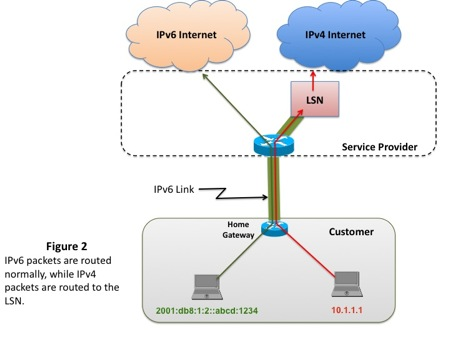
\includegraphics[width=150px]{img/img2.jpg}
	\end{figure}
    \column{0.5\textwidth}
	 \begin{itemize}
		\item
			Un mensaje IPv6 se envía normalmente.
		\item
			Si el mensaje va en IPv4 se utiliza la 
			técnica mencionada anteriormente. Es decir, 
			el paquete IPv4 encapsulado en uno IPv6 y 
			enviado a un LSN disponible.
	\end{itemize}
  \end{columns}
\end{frame}

\begin{frame}
  \frametitle{Problemas}
  	\begin{itemize}[itemsep=2em]
		\item
			La funcionalidad que permite el paso de mensajes
			en IPv4 a través de IPv6 debe ser implementada
			en los equipos locales.
		\item
			En general las ISP son reacias a molestar a los
			usuarios, por lo que la estrategia consistiría
			en implementar el método en los nuevos clientes
			y a medida que se renueven los equipos.
	\end{itemize}
\end{frame}

\begin{frame}
  \frametitle{Esquema ideal}
  \begin{columns}[t]
    \column{0.5\textwidth}
    	\begin{figure}
		\centering
		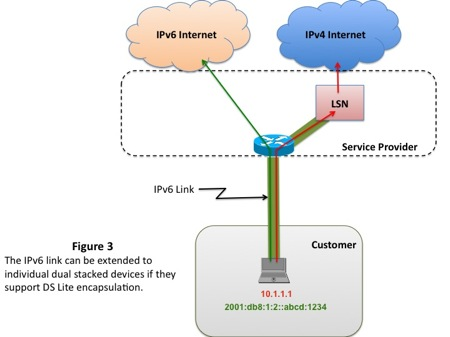
\includegraphics[width=150px]{img/img3.jpg}
	\end{figure}
    \column{0.5\textwidth}
    	\begin{itemize}[itemsep=2em]
		\item
			Dual Stack implementado en los equipos.
		\item
			Los equipos son capaces de interactuar
			con ambos protocolos.
	\end{itemize}
  \end{columns}
\end{frame}







\section{socket.h}
\subsection{Descripción}

\begin{frame}
	\frametitle{Recuerdo.}
	\begin{itemize}[itemsep=2em]
	\item
		Provee funciones básicas para el traspaso de paquetes vía socket.
	\item
		Soporta los protocolos de transporte \texttt{UDP} y \texttt{TCP}.
	\item
		Soporta los protocolos de red IPv4 y IPv6.
	\item
		Nos enfocaremos en el traspaso de mensajes \texttt{TCP/IP} tanto
		versión 4 como 6.
	\end{itemize}
% Mini bloques dentro de las ppt
%\begin{block}{Marsupiales en Australia}
% Koala, Canguro, Wombat...
%\end{block}			 
\end{frame}

\subsection{Funcionalidad}

\begin{frame}[fragile]
	\frametitle{Creación del socket}
	\begin{verbatim}
	#include <sys/socket.h>
	/* int = socket(int domain, int type, int protocol); */
	int mi_socket;
	mi_socket = socket(AF_INET, SOCK_STREAM, IPPROTO_TCP);
	\end{verbatim}
	\begin{itemize}
		\item
			\texttt{domain}: dominios de transmisión, puede ser
			\texttt{AF\_INET} en el caso de IPv4, \texttt{AF\_UNIX} para
			comunicación interna, etc.
		\item
			\texttt{type}: Tipo de conexión, \texttt{SOCK\_STREAM} para 
			\texttt{TCP} o \texttt{SOCK\_DGRAM} para \texttt{UDP}.
		\item
			\texttt{protocol}: Protocolo utilizado. Si el tipo (\texttt{type}) 
			solo tiene un protocolo se puede poner un 0 (ej: \texttt{TCP}).
	\end{itemize}
\end{frame}

\begin{frame}
	\centering
	\adjustbox{max height=\dimexpr\textheight-5.5cm\relax,max width=\textwidth}{
	\begin{tabular}{|c|c|}
		\hline
		\textbf{domain} & \textbf{Descripción} \\
		\hline
		\texttt{AF\_UNIX} & Comunicación interna Unix.\\
		\hline
		\texttt{AF\_INET} & Comunicación IPv4.\\
		\hline
		\texttt{AF\_INET6} & Comunicación IPv6.\\
		\hline
		\texttt{AF\_APPLETALK} & Comunicación para AppleTalk. \\
		\hline
		\hline 
		\textbf{type}& \textbf{Descripción} \\
		\hline
		\texttt{SOCK\_STREAM} & Socket de flujos, orientado a la conexión. \\
		\hline
		\texttt{SOCK\_DGRAM} & Socket de datagramas, envía los paquetes
		individualmente. \\
		\hline
		\texttt{SOCK\_SEQPACKET} & Envia los paquetes secuencialmente. \\
		\hline
		\texttt{SOCK\_RDM} & Socket de datagramas, confiable pero no ordenado.\\
		\hline
	\end{tabular}
}\\[0.4cm]
	\small Una vez elegido el tipo de socket que queremos utilizar debemos
	ligarlo a nuestra dirección y puerto. Las estructuras de IPv4 y IPv6 son
	diferentes.
\end{frame}

\begin{frame}[fragile]
	\frametitle{Comparación es estructuras.}
	Estructura IPv4:
	\small
	\begin{verbatim}
struct in_addr {
    unsigned long s_addr;  // Dirección IPv4
};

struct sockaddr_in {
    short            sin_family;   // Dominio AF_INET.
    unsigned short   sin_port;     // Puerto
    struct in_addr   sin_addr;     // Dirección IPv4.
    char             sin_zero[8];  // Ceros.
};
	\end{verbatim}
\end{frame}

\begin{frame}[fragile]
	\frametitle{Comparación es estructuras.}
	Estructura IPv6:
	\small
	\begin{verbatim}
struct in6_addr {
    u_int8_t  s6_addr[16];  // Dirección IPv6
}

struct sockaddr_in6 {
    u_char           sin6_len;      // Largo de esta estructura.
    u_char           sin6_family;   // Dominio AF_INET6.
    u_int16m_t       sin6_port;     // Puerto.
    u_int32m_t       sin6_flowinfo; // Cero.
    struct in6_addr  sin6_addr;     // Dirección IPv6.
};
	\end{verbatim}
\end{frame}

\begin{frame}[fragile]
	\frametitle{Convenciones.}
	En las estructuras vistas, los campos para manejar el puerto y la dirección 
	utilizan un ordenamiento de bytes especial (formato network) para guardar
	la información, por ello se hacen necesarias funciones de conversión.
	\begin{verbatim}
	// Para la dirección IP:
	int inet_pton(int af, const char *cp, void *buf);
	/* af: AF_INET o AF_INET6, 
	 * cp: dirección IPv4 o IPv6, 
	 * buf: buffer para el resultado. */

	// Para el puerto:
	uint16_t htons(uint16_t hostshort);
	// hostshort: Puerto.
	\end{verbatim}
\end{frame}

\begin{frame}[fragile]
	Una vez configurado el socket y la estructura de dirección, debemos crear
	la relación entre ellos:
	\begin{verbatim}
	int bind(int fd, struct sockaddr *addr, int addrlen);
	/* fd: Descriptor del socket,
	 * addr: Estructura de dirección,
	 * addrlen: Largo de la estructura de dirección. */
	\end{verbatim}
	Con nuestro sockey y dirección configurados podemos intentar establecer una
	conexión (\texttt{connect();}) con un servidor que debe estar en ``modo 
	escucha'' (\texttt{listen();}). Este ultimo debe aceptar la conexión 
	(\texttt{accept();}) antes de poder enviar y recibir mensajes
	(\texttt{send();} y \texttt{recv();}).
\end{frame}

\begin{frame}[fragile]
	\frametitle{Funciones importantes.}
	\small
	\begin{verbatim}
	int listen(int fd, int backlog);
	/* fd: descriptor del socket,
	 * backlog: numero de conexiones permitidas. */ 
	
	int connect(int fd, struct sockaddr *server, int addrlen);
	/* server: estructura de dirección del servidor */

	int accept(int fd, void *addr, int *addrlen);
	/* addr: puntero para la dirección de quien nos contacta. */

	int send(int fd, const void *msg, int len, int flags);
	/* msg: puntero a los datos que queremos enviar */

	int recv(int fd, void *buf, int len, unsigned int flags);
	/* buf: buffer para guardar los datos */
	\end{verbatim}
\end{frame}

\begin{frame}[fragile]
	\frametitle{Terminando la conexión.}
	Una vez enviados los paquetes debemos cerrar los sockets.
	\small
	\begin{verbatim}
	int shutdown(int fd, int how);
	/* fd: descriptor del socket,
	 * how: 0 para prohibir la recepción,
	        1 para prohibir el envío,
	        2 para prohibir ambos. */
	
	/* Utilizar how=2  es equivalente a close() */
	close(fd);
	\end{verbatim}
\end{frame}
\end{document}
